\newpage\setcounter{section}{4}
\section{Submanifolds}

The bulk of this chapter will be focused on the most important type of submanifolds: embedded submanifolds. There have the subspace topology inherited from their containing manifold, and turn out to be exactly the images of smooth embeddings. The other type of submanifold we will discuss, immersed submanifolds, are slightly less nice objects since they are not required to have the subspace topology, but as you would expect, they appear as the images of injective immersions.

\subsection{Embedded and Immersed Submanifolds}\nl

\dfn An \df{embedded submanifold of M} is a subset $S\seq M$ that is a manifold in the subspace topology, endowed with a smooth structure with respect to which the inclusion map $S\into M$ is a smooth embedding. Embedded submanifolds are also called \df{regular submanifolds} by some.

\dfn If $S$ ins an embedded submanifold of $M$, the \df{codimension of S in M} is given by $\dim(M) - \dim(S)$. $M$ is called the \df{ambient manifold} for $S$, and an embedded submanifold of codimension one is called an \df{embedded hypersurface}.

\begin{prop}[Open Submanifolds]
Suppose $M$ is a smooth manifold. The embedded submanifolds of codimension 0 in $M$ are exactly the open submanifolds.
\end{prop}

\begin{prop}[Images of Embeddings as Submanifolds]
Suppose $M$ is a smooth manifold with or without boundary, $N$ is a smooth manifold, and $F:N\ra M$ is a smooth embedding. Let $S = F(N)$. With the subspace topology, $S$ is a topological manifold, and it has a unique smooth structure making it into an embedded submanifold of $M$ with the property that $F$ is a diffeomorphism onto its image.
\end{prop}

\setcounter{thm}{3}

\begin{prop}[Graphs as Submanifolds]
Suppose $M$ is a smooth $m$-manifold (without boundary), $N$ is a smooth $n$-manifold with or without boundary, $U\seq M$ is open, and $f:U\ra N$ is a smooth map. Let $\Gamma(f)\seq M\times N$ denote the graph of $f$:
\[\Ga(f) = \{(x,y)\in M\x N\ :\ x\in U, y = f(x)\}.\]
Then $\Ga(f)$ is an embedded $m$-dimensional submanifold of $M\x N$.
\end{prop}

\begin{center}
    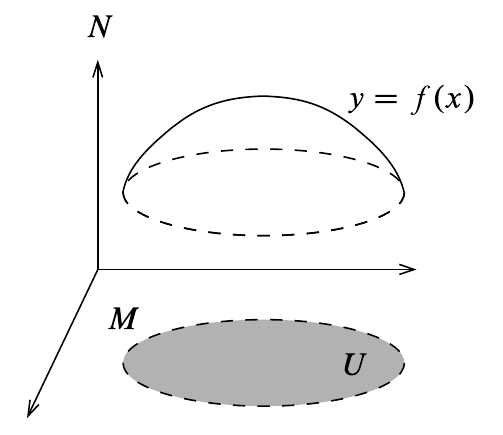
\includegraphics[scale = 0.5]{chapter05/c5f1.png}
\end{center}

\dfn An embedded submanifold $S\seq M$ is said to be \df{properly embedded} if the inclusion $S\into M$ is a proper map.

\begin{prop}
Suppose $M$ is a smooth manifold \wowob and $S\seq M$ is an embedded submanifold. Then $S$ is properly embedded if and only if it is a closed subset of $M$.
\end{prop}

\begin{cor}
Every compact embedded submanifold is properly embedded.
\end{cor}

\dfn If $Y$ is an open subset of $\Rn$ and $k\in \{0,\ldots,n\}$, a \df{k-dimensional slice of U} (or simply a \df{k-slice}) is any subset of the form 
\[S = \{(x^1,\ldots,x^k,x^{k + 1},\ldots, x^n)\in U\ :\ x^{k + 1} = c^{k + 1},\ldots,x^n = c^n\}\]
for some constants $c^{k + 1},\ldots,c^n$.

\dfn Let $M$ be a smooth $n$-manifold, and let $(U,\vphi)$ be a smooth chart on $M$. If $S$ is a subset of $U$ such that $\vphi(S)$ is a $k$-slice of $\vphi(U)$, the we say that \df{S is a k-slice of U}.

\dfn Given a subset $S\seq M$ and a nonnegative integer $k$, we say that $S$ satisfies the \df{\hlb{local k-slice condition}} if each point of $S$ is contained in the domain of a smooth chart $(U, \vphi)$ for $M$ such that $S\cap U$ is a single $k$-slice in $U$. Any such chart is called a \df{slice chart for S in M}, and the corresponding coordinates $(x^1,\ldots,x^n)$ are called \df{slice coordinates}.

\setcounter{thm}{7}

\begin{thm}[\hlb{Local Slice Criterion for Embedded Submanifolds}]
Let $M$ be a smooth $n$-manifold. If $S\seq M$ is an embedded $k$-dimensional submanifold, then $S$ satisfies the local $k$-slice condition, then with the subspace topology, $S$ is a topological manifold of dimension $k$, and it has a smooth structure making it into a $k$-dimensional embedded submanifold of $M$.
\end{thm}

\begin{ex}[Spheres as Submanifolds]
For any $n\geq 0$, $\BSN$ is an embedded submanifold of $\R^{n + 1}$, because it is locally the graph of a smooth function: as is shown in Example 1.4 of Lee, the intersection of $\BSN$ with the open subset $\{x\ :\ x^i > 0\}$ is the graph of the smooth function
\[x^i = f(x^1, \ldots, x^{i - 1}, x^{i + 1}, \ldots, x^{n + 1}),\]
where $f:\B^n\ra \R$ is given by $f(u) = \sqrt{1 - |u|^2}$. Similarly, the intersection of $\BSN$ with $\{x\ :\ x^i < 0\}$ is the graph of $-f$. Since every point in $\BSN$ is in one of these sets, $\BSN$ satisfies the local $n$-slice condition and is thus an embedded submanifold of $\R^{n + 1}$. The smooth structure thus induced on $\BSN$ is the same as the one we defined in Chapter 1: in fact, the coordinates for $\BSN$ determined by these slice charts are exactly the graph coordinates defined in Example 1.31 of Lee.
\end{ex}

\setcounter{thm}{10}

\begin{thm}
If $M$ is a smooth $n$-manifold with boundary, then with the subspace topology, $\bd M$ is a topological $(n - 1)$-dimensional manifold (without boundary), and has a smooth structure such that it is a properly embedded submanifold of $M$.
\end{thm}

\dfn If $\Phi:M\ra N$ is any map and $c$ is any point of $N$, we call the set $\Phi\inv(c)$ a \df{level set of $\boldsymbol{\Phi}$}.

\setcounter{thm}{11}

\begin{thm}[\hlb{Constant-Rank Level Set Theorem}]
Let $M$ and $N$ be smooth manifolds, and let $\Phi:M\ra N$ be a smooth map with constant rank $r$. Each level set of $\Phi$ is a properly embedded submanifold of codimension $r$ in $M$.
\end{thm}

\begin{cor}[Submersion Level Set Theorem]
If $M$ and $N$ are smooth manifolds and $\Phi:M\ra N$ is a smooth submersion, then each level set of $\Phi$ is a properly embedded submanifold whose codimension is equal to the dimension of $N$.
\end{cor}

\dfn If $\Phi:M\ra N$ is a smooth map, a point $p\in M$ is said to be a \df{regular point of $\boldsymbol{\Phi}$} if $d\Phi_p:T_pM\ra T_{\Phi(p)}N$ is surjective; it is a \df{critical point of $\boldsymbol{\Phi}$} otherwise.

\dfn A point $c\in N$ is said to be a \df{regular value of $\boldsymbol{\Phi}$} if every point of the level set $\Phi\inv(c)$ is a regular point, and a\df{critical value} otherwise. In particular, if $\Phi\inv(c) = \es$, then $c$ is a regular value. Finally, a level set $\Phi\inv(c)$ is called a \df{regular level set} if $c$ is a regular value of $\Phi$.

\begin{cor}[\hlb{Regular Level Set Theorem}]
Every regular level set of a smooth map between smooth manifolds is a properly embedded submanifold whose codimension is equal to the dimension of the codomain.
\end{cor}

\begin{ex}[\hlo{Spheres}]
Now we can give a much easier proof that $\BSN$ is an embedded submanifold of $\R^{n + 1}$. The sphere is a regular level set of the smooth function $f:\R^{n + 1}\ra R$ given by $f(x) = |x|^2$, since $df_x(v) = 2\sum_ix^iv^i$, which is surjective except at the origin.
\end{ex}

\begin{prop}
Let $S$ be a subset of a smooth $m$-manifold $M$. Then $S$ is an embedded $k$-submanifold of $M$ if and only if every point of $S$ has a neighborhood $U$ in $M$ such that $U\cap S$ is a level set of a smooth submersion $\Phi:U\ra \R^{m - k}$.
\end{prop}

\begin{center}
    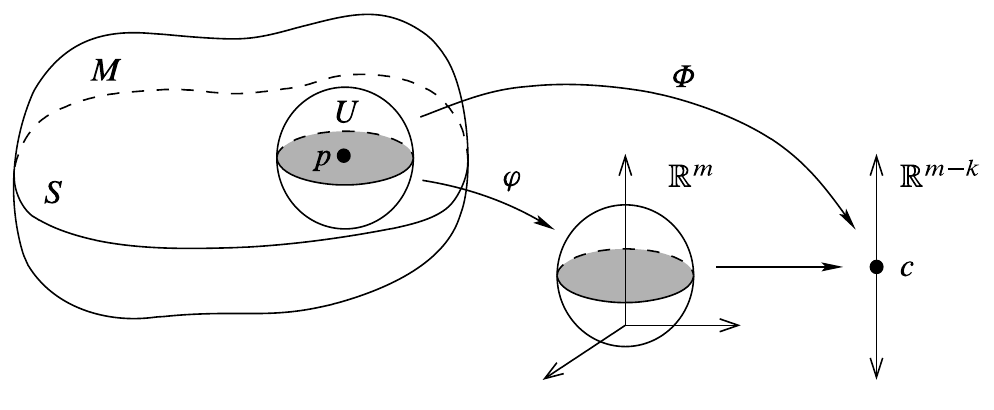
\includegraphics[scale = 0.43]{chapter05/c5f6.png}
\end{center}

\dfn If $S\seq M$ is an embedded submanifold, a smooth map $\Phi:M\ra N$ such that $S$ is a regular level set of $\Phi$ is called a \df{defining map for S}. More generally, if $U$ is an open subset of $M$ and $\Phi:U\ra N$ is a smooth map such that $S\cap U$ is a regular level set of $\Phi$, the $\Phi$ is called a \df{local defining map for S}.

\dfn An \df{\hl{immersed submanifold of M}} is a subset $S\seq M$ endowed with a topology with respect to which it is a topological manifold (without boundary), and a smooth structure with respect to which the inclusion map $S\into M$ is a smooth immersion. As for embedded submanifolds, we define the \df{codimension of S in M} to be $\dim(M) - \dim(S)$.

\setcounter{thm}{17}

\begin{prop}[\hl{Images of Immersions as Submanifolds}]
Suppose $M$ is a smooth manifold \wowob, $N$ is a smooth manifold, an d$F:N\ra M$ is an injective smooth immersion. Let $S = F(N)$. Then $S$ has a unique topology and smooth structure such that it is a smooth submanifold of $M$ and such that $F:N\ra S$ is a diffeomorphism onto its image.
\end{prop}

\setcounter{thm}{20}

\begin{prop}
Suppose $M$ is a smooth manifold \wowob, and $S\seq M$ is an immersed submanifold. If any of the following holds, then $S$ is embedded.
\begin{enumerate}
    \item $S$ has codimension 0 in $M$.
    \item The inclusion map $S\seq M$ is proper.
    \item $S$ is compact.
\end{enumerate}
\end{prop}

\begin{prop}[Immersed Submanifolds Are Locally Embedded]
If $M$ is a smooth manifold with or without boundary, and $S\seq M$ is an immersed submanifold, then for each $p\in S$ there exists a neighborhood $U$ of $p$ in $S$ that is an embedded submanifold of $M$.
\end{prop}

\dfn Suppose $X\seq M$ is an immersed $k$-dimensional submanifold. A \df{local parameterization of S} is a continuous map $X:U\ra M$ whose domain is an open subset $U\seq \Rk$, whose image is an open subset of $S$, and which, considered as a map into $S$, is a homeomorphism onto its image. It is called a \df{smooth local parameterization} if it is a diffeomorphism onto its image. If the image of $X$ is all of $S$, it is called a \df{global parameterization}.

\begin{prop}
Suppose $M$ is a smooth manifold with or without boundary, $S\seq M$ is an immersed $k$-submanifold, $\iota:S\into M$ is the inclusion map, and $U$ is an open subset of $\Rk$. A map $X:U\ra M$ is a smooth local parameterization of $S$ if and only if there is a smooth coordinate chart $(V,\vphi)$ for $S$ such that $X = \iota\circ\vphi\inv$. \hl{Therefore, every point of $S$ is the image of some local parametrization.}
\end{prop}

\setcounter{thm}{26}

\begin{thm}[Restricting the Domain of a Smooth Map]
If $M$ and $N$ are smooth manifold with or without boundary, $F:M\ra N$ is a smooth map, and $S\seq M$ is an immersed or embedded submanifold, then $F|_S:S\ra N$ is smooth.
\end{thm}

\setcounter{thm}{28}

\begin{thm}[Restricting the Codomain of a Smooth Map]
Suppose $M$ is a smooth manifold (without boundary), $S\seq M$ is an immersed submanifold, and $F:N\ra M$ is a smooth map whose image is contained in $S$. If $F$ is continuous as a map from $N$ to $S$, then $F:N\ra S$ is smooth.
\end{thm}

\begin{center}
    \includegraphics[scale = 0.38]{chapter05/c5f9.png}
\end{center}

\begin{cor}[\hl{Embedded Case}]
Let $M$ be a smooth manifold and $S\seq M$ be an embedded submanifold. Then every smooth map $F:N\ra M$ whose image is contained in $S$ is also a smooth map from $N$ to $S$.
\end{cor}

\begin{thm}
Suppose $M$ is a smooth manifold and $S\seq M$ is an embedded submanifold. \hl{The subspace topology on $S$ and the smooth structure described in Theorem 5.8 are the only topology and smooth structure with respect to which $S$ is an embedded or immersed submanifold.}
\end{thm}

\begin{thm}
Suppose $M$ is a smooth manifold and $S\seq M$ is an immersed submanifold. For the given topology on $S$, there is only one smooth structure making $S$ into an immersed submanifold.
\end{thm}

\setcounter{thm}{33}

\begin{lem}[\hlb{Extension Lemma for Functions on Submanifolds}]
Suppose $M$ is a smooth manifold, $S\seq M$ is a smooth submanifold, and $f\in \Cin(S)$.
\begin{enumerate}
    \item If $S$ is embedded, then there exists a neighborhood $U$ of $S$ in $M$ and smooth function $\td f\in \Cin(U)$ such that $\td f|_S = f$.
    \item If $S$ is properly embedded, then the neighborhood $U$ in part (a) can be taken to be all of $M$.
\end{enumerate}
\end{lem}

\newpage
\subsection{Tangent Space to a Submanifold}\nl

\dfn Let $M$ be a smooth manifold with or without boundary, and let $S\seq M$ be an immersed or embedded submanifold. Since the inclusion map $\iota:S\into M$ is a smooth immersion, at each point $p\in S$ we have an injective linear map $d\iota_p:T_pS \ra T_pM$. We adopt the convention of identifying $T_pS$ with its image under this map, thereby thinking of $T_pS$ as a certain linear subspace of $T_pM$.

\begin{center}
    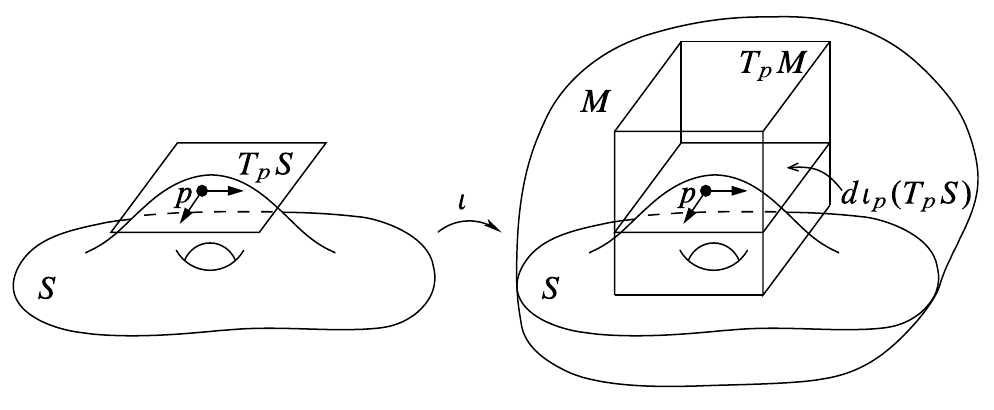
\includegraphics[scale = 0.45]{chapter05/c5f12.png}
\end{center}

\begin{prop}
Suppose $M$ is a smooth manifold \wowob, $S\seq M$ is an immersed or embedded submanifold, and $p\in S$. A vector $v\in T_pM$ is in $T_pS$ if and only if there is a smooth curve $\ga:J\ra M$ whose image is contained in $S$, and which is also smooth as a map into $S$, such that $0\in J,\ga(0) = p$, and $\ga\p(0) = v$.
\end{prop}

\setcounter{thm}{36}

\begin{prop}
Suppose $M$ is a smoth manifold, $S\seq M$ is an embedded submanifold, and $p\in S$. As a subspace of $T_pM$, the tangent space $T_pS$ is characterized by
\[T_pS = \{v\in T_pM\ :\ vf = 0\text{ whenever $f\in \Cin(M)$ and }f|_S = 0\}.\]
\end{prop}

\begin{prop}
Suppose $M$ is a smooth manifold and $S\seq M$ is an embedded submanifold. If $\Phi:U\ra N$ is any local defining map for $S$, then $T_pS = \ker(d\Phi_p):T_pM\ra T_{\Phi(p)}N$ for each $p\in S\cap U$.
\end{prop}

\begin{cor}
Suppose $S\seq M$ is a level set of a smooth submersion $\Phi = (\Phi^1,\ldots,\Phi^k):M\ra \Rk$. A vector $v\in T_pM$ is tangent to $S$ if and only if $v\Phi^1= \cdots = v\Phi^k = 0$.
\end{cor}


\hlb{\textbf{Note:}} In general there are several good strategies for showing $S\seq M$ is \textit{not} an immersed. Here are some useful facts to keep in mind:
\begin{enumerate}
    \item If $S$ is immersed, then $T_pS$ is a linear subspace of $T_pM$ of the same dimension at every $p\in S$
    \item Every $p\in S$ must be the image of some local parameterization $X:U\ra S$.
    \item Every $v\in T_pS$ is the velocity vector of some curve in $S$.
    \item \hl{Every tangent vector of $S$ annihilates every smooth function on $M$ that is constant on $S$.}
\end{enumerate}